\documentclass{article}
\usepackage{multirow}
\usepackage{array}
\usepackage{tikz}
\usepackage{geometry}
\geometry{margin=1in}
\begin{document}

Table 1 : \\

\setlength{\extrarowheight}{7pt}
\begin{tabular}{|c|c|c|c|}
\hline
A & \multicolumn{3}{c|}{C} \\
\hline
\multirow{2}{*}{B} & \multirow{2}{*}{D} & \multirow{2}{*}{E} & F \\
\cline{4-4}
 &  &  & G \\
\hline
\multicolumn{4}{|c|}{H} \\
\hline
\multicolumn{4}{|c|}{I} \\
\hline 
\end{tabular} \\ \\

Table 2 : \\

\setlength{\extrarowheight}{10pt}
\begin{tabular}{|c|c|c|c|}
\hline
\multicolumn{2}{|c|}{P} & \multicolumn{2}{c|}{R} \\
\hline
\multicolumn{2}{|c|}{Q} & \multicolumn{2}{c|}{S} \\
\hline
T & V & X & \multirow{2}{*}{Z}\\
\cline{1-3}
U & W & Y &  \\
\hline

\end{tabular} \\ \\

Table 3 : \\

\setlength{\extrarowheight}{7pt}
\begin{tabular}{|c|c|c|c|}

\hline
\multirow{3}{*}{J} & \multirow{3}{*}{K} & \multirow{3}{*}{L} & M \\
\cline{4-4}
 &  &  & N \\
\cline{4-4}
 &  &  & O \\
\hline
\end{tabular} \\ \\

Table 4 : \\

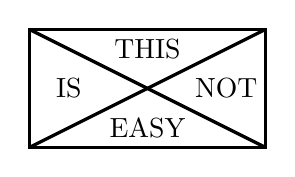
\begin{tikzpicture}[scale=0.5]
    % Draw the rectangle border
    \draw[very thick] (0,0) rectangle (6,3);

    % Draw diagonals
    \draw[very thick] (0,0) -- (6,3);
    \draw[very thick] (0,3) -- (6,0);

    % Add the text
    \node at (3,2.5) {THIS};
    \node at (1,1.5) {IS};
    \node at (5,1.5) {NOT};
    \node at (3,0.5) {EASY};
\end{tikzpicture} \\

Combining 3 tables : \\

\setlength{\extrarowheight}{20pt}
\begin{tabular}{cc}
 \setlength{\extrarowheight}{7pt}
\begin{tabular}{|c|c|c|c|}
\hline
A & \multicolumn{3}{c|}{C} \\
\hline
\multirow{2}{*}{B} & \multirow{2}{*}{D} & \multirow{2}{*}{E} & F \\
\cline{4-4}
 &  &  & G \\
\hline
\multicolumn{4}{|c|}{H} \\
\hline
\multicolumn{4}{|c|}{I} \\
\hline 
\end{tabular}  &
\noindent
\makebox[0pt][l]{
\hspace{-0.9cm}
\setlength{\extrarowheight}{12pt}
\begin{tabular}{|c|c|c|c|}
\hline
\multicolumn{2}{|c|}{P} & \multicolumn{2}{c|}{R} \\
\hline
\multicolumn{2}{|c|}{Q} & \multicolumn{2}{c|}{S} \\
\hline
T & V & X & \multirow{2}{*}{Z}\\
\cline{1-3}
U & W & Y &  \\
\hline
\end{tabular} } \\
\raisebox{2.85cm}{
\makebox[0pt][l]{
\hspace{-1.7cm}
 \setlength{\extrarowheight}{1.5pt}
\begin{tabular}{|c|c|c|c|}
\hline
\multirow{3}{*}{J} & \multirow{3}{*}{K} & \multirow{3}{*}{L} & M \\
\cline{4-4}
 &  &  & N \\
\cline{4-4}
 &  &  & O \\
\hline
\end{tabular} } } & 
\raisebox{2.2cm}{
\makebox[0pt][l]{
\hspace{-0.82cm}
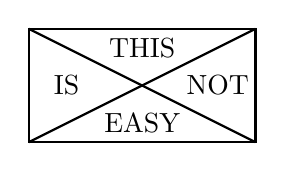
\begin{tikzpicture}[scale=0.48]
    % Draw the rectangle border
    \draw[thick] (0,0) rectangle (6,3);

    % Draw diagonals
    \draw[thick] (0,0) -- (6,3);
    \draw[thick] (0,3) -- (6,0);

    % Add the text
    \node at (3,2.5) {THIS};
    \node at (1,1.5) {IS};
    \node at (5,1.5) {NOT};
    \node at (3,0.5) {EASY};
\end{tikzpicture} } } \\
\end{tabular}


\end{document}




















